% !TEX encoding = UTF-8
% !TEX TS-program = pdflatex
% !TEX root = ../thesis.tex

\chapter{Introduction}
This chapter introduces the problem: what we are analyzing, why 
this problem exists, how it is defined, and how it can be resolved. 
Also we present the company, the internship, and the work 
methodology.
% /*//////////////////////////////////////////////////////////////
%                           THE PROBLEM
% //////////////////////////////////////////////////////////////*/
\section{The problem}
As stated in the abstract, the main problem is preserving the ownership 
of people's data. In order to achieve this objective, we pass through 
problems like interoperability, privacy safeguarding, law compliance, security,
and others.
\vspace*{0.3cm}\\
First, let us very quickly present Self-Sovereign Identity (we analyze it more 
thoroughly in the following chapters): this concept digitalizes people's credentials
(e.g., their identity card), introducing Verifiable Credentials. These, as the 
physical correspondings, are held by the people, issued by some authorized entity,
and verified by other bodies.
\vspace*{0.3cm}\\
Assuming we can create a system where people hold their digital credentials:
\begin{enumerate}
    \setlength\itemsep{-0.3em}
    \item \textbf{Interoperability}: how can these credentials be shown to and 
    verified in the same manner by different actors?
    \item \textbf{Privacy}: can we demonstrate something without revealing it, 
    preserving our privacy this way?
    \item \textbf{Law compliance}: is it possible to save on blockchain people's
    data, or are we going against specific privacy laws?
    \item \textbf{Security}: are credentials susceptible to attacks from hackers 
    trying to steal our data?
\end{enumerate}
Thanks to Self-Sovereign Identity, we can give a positive answer to all
of these questions, but as is often the case, we have to deal with 
compromises.

\paragraph{Worldwide scenario.} The current situation is clear. Every time we 
find a new website, we may want to interact with it, and to do so, we 
have to register to create a profile. In this phase, we have to give our data to 
the company, and they will be stored in their databases.

\paragraph{Problem identification.} Let us now try to answer the previous questions 
to check how the present context is managed:
\begin{enumerate}
    \item \textbf{Interoperability}: we could have two cases. In the first one, 
    we use a technology that enables us to use our existing account on 
    multiple websites, which integrates this solution, for example, "Sign-Up 
    with Google". Here our data is owned by Google, which shares them (if we 
    grant permission) with third parties, and no one prohibits third parties 
    from keeping our shared data saved. In the second case, we must register 
    each time if the third party does not integrate other "Sign-Up with \textbf{*}" 
    solutions. In both cases, third parties can collect our data (in the 
    first case, Google explicitly knows our interests, but there is a minimum
    degree of interoperability). Also, in most cases, companies will let us 
    create multiple accounts without verifying our data (one exception to 
    this is the use of \acrshort{kyc}).
    \item \textbf{Privacy}: in some cases, we must show our data
    with complete transparency: for example, the police stop us on the 
    street and ask for our details. Nevertheless, let us suppose we want to 
    demonstrate something without revealing the details. For example, 
    someone has graduated and wants to demonstrate it without revealing 
    his final grade. We can do this thanks to a cryptography method 
    called \textit{Zero-Knowledge Proof}\cite{article:zkp}. However, this has not yet been
    implemented in most current systems.
    \item \textbf{Law compliance}: if we consider saving users' data in 
    blockchains, this problem does not exist as we examine centralized 
    systems which do not use them. By the way, of course, there are privacy 
    laws companies must follow (like \acrshort{gdpr}).
    \item \textbf{Security}: our information is stored in databases. With 
    a data breach, considering a centralized system, a malicious actor can 
    access all users' data at once. Sadly, this happens often. So often 
    that someone has made a website where anyone can check if his data has 
    been stolen online at least once\cite{site:pwned}.
\end{enumerate}

\paragraph{Problem statement.} With the above considerations, it is clear that 
the existing systems work but could be significantly improved. In fact, 
interoperability enhancement would mean privacy and security penalization. 
Compromises exist, but if the system is well designed, they can be significantly 
reduced or at least moved to less dangerous areas. Here, the need for a more 
secure way to store user data arises. A way that intersects the analyzed points, 
bringing new power to people and reducing that of companies. This is the 
Self-Sovereign Identity principle, which the developed solution leverages.

\paragraph{Approaches.} SSI concept\cite{site:sovrinssi} is pretty simple, as opposed to its 
(in development) implementation. Everyone has different relationships or 
unique sets of identifying information. This information could include 
birth date, citizenship, university degrees, or business licenses. In the 
physical world, these are represented as cards and certificates that the 
citizen holds in their wallet or a secure place like a safety deposit 
box. They are presented when the person needs to prove their identity or 
something about it. Self-sovereign identity (SSI) brings the same freedom and 
personal autonomy to the internet in a safe and trustworthy identity management 
system. SSI means the individual (or organization) manages the elements that 
make up their identity, and he digitally controls access to those credentials,
called Verifiable Credentials (or \acrshort{vc}s). They are digital representations of
information that can be verified by a third party.
\vspace*{1cm}\\
This is achievable by involving three participants:
\begin{enumerate}
    \item \textbf{Holder}: the holder is an individual in the scenario, 
    although it can also be an organization/company. The holder is the 
    entity that holds the credential\footnote{Not always the holder and 
    credential's subject coincide: for example, someone could hold a verifiable 
    credential of his dog.}.
    \item \textbf{Issuer}: the issuer is the institution, be it a company, 
    certifier body, or governmental organization, that has been awarded a 
    level of trust to provide information (i.e., a public body that issued 
    a passport)
    \item \textbf{Verifier}: the verifier is the individual, organization,
    company, or government with whom the holder must prove information's 
    legitimacy and trustworthiness.
\end{enumerate}
The \acrfull{vdr} grants the trust: here are stored schemas and 
identifiers (linked to the credentials) that the verifiers use to check 
data validity without the issuer's intervention.
\vspace*{0.3cm}\\
To make a preliminary check of this solution's viability, let us try to 
answer the previous four questions, considering the new scenario:
\begin{enumerate}
    \item \textbf{Interoperability}: with standards definition, credentials
    can be presented to verifiers by holders, in the same manner each time. 
    Examples of standards could be credentials schemas (e.g., defining which fields are 
    mandatory) and verification policies (i.e., how the credentials are verified).
    \item \textbf{Privacy}: as already stated, we can demonstrate something
    without revealing its details with \textit{Zero-Knowledge Proofs}. This 
    technology has already found applications and implementations in 
    blockchains (e.g., mixers\cite{site:mixers}, zk-rollups\cite{site:zkrollups}, 
    or zk-games like Dark Forest\cite{site:darkforest}), 
    so a decentralized system that leverages \acrshort{zkp}s is buildable.
    \item \textbf{Law compliance}: as can be read later in the paper, 
    this is one of the most challenging points of the full SSI integration 
    with blockchains because of its transparency nature. Everything is 
    registered and immutable, so we must choose what to register and what 
    not. Again, compromises are needed.
    \item \textbf{Security}: as users hold credentials, as long as they are
    not saved in centralized servers, significant data breaches (targeting 
    databases) would happen way less often. The user is responsible for his 
    information security, and secure communication protocols enhances it.
\end{enumerate}
After quickly drafting these reflections, it can be said that SSI 
principles fit our problem requests, so a solution that aims to solve them 
can be tried to be developed.\\
These analyzed points are well discussed in an article by Christopher Allen 
called "The path to Self-Sovereign Identity", where he defines the "Ten 
Principles of Self-Sovereign Identity"\cite{site:ssiprinciples}.

% /*//////////////////////////////////////////////////////////////
%                           USE CASES
% //////////////////////////////////////////////////////////////*/
\section{Basic use cases}
After addressing the problem and trying to provide answers to the initial 
questions, it is possible to start thinking about the first use cases.
Obviously, the minimum requirement is credentials involvement: each time a user 
has to demonstrate some information, SSI could theoretically be leveraged.
\vspace*{0.3cm}\\
In the first part of the internship, the focus has been (after the SSI primitives 
study) on use cases. They can be grouped into these two macro-categories:
\paragraph{Academics.}
Here we can include all the uses about, for instance, university. A lot of them 
can be thought about and analyzed, but the most interesting which have been examined 
are these:
\begin{enumerate}
    \item \textbf{Exams and Diplomas emission}: students can present 
    their credentials (badge) to the university to register for exams. 
    Each exam result would be another credential, and in order to access the 
    diploma, he should present all the credentials related to passed exams 
    (possibly wrapping them in a "presentation"). The final diploma would 
    be another Verifiable Credential emitted by the university.
    \item \textbf{Scholarships requests}: students can demonstrate they are 
    eligible for facilitations by presenting their credentials to the university. 
    This way, information pieces are easily checkable and verifiable, and procedures 
    would be faster and less susceptible to errors. A "permit" credentials could be 
    emitted, which would grant the student access to facilitations (e.g., canteen,  
    money, discounts...)
    \item \textbf{Discounts and university canteen}: it is evident that comfortable
    functions come into effect by processing the previous use case. Instead of 
    creating accounts with university e-mail, students should present their 
    credentials to services that offer facilitations, bringing interoperability 
    and trust to each part. Figure 1.1 shows a possible scenario.
\end{enumerate}
\begin{center}
    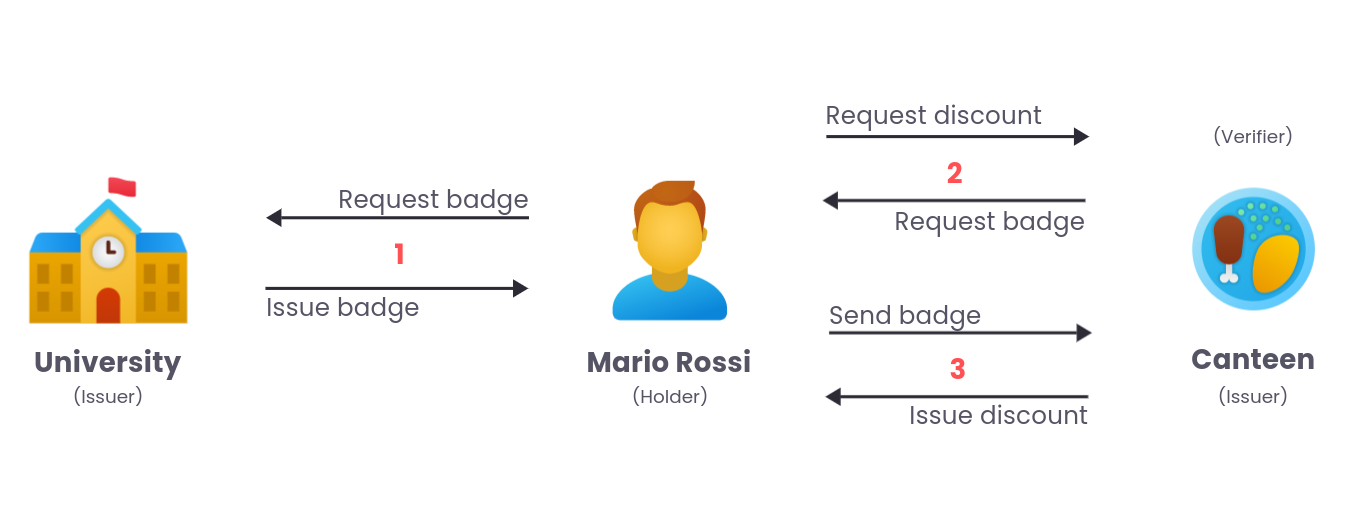
\includegraphics[scale=0.25]{chapter1/universityUc.png}
    \captionof{figure}{University canteen use case}
\end{center}
    
\paragraph{Institutionals.}
Here we can place all use cases involving the participation of national, 
European (or other unions), or global entities.
Noteworthy examples are:
\begin{enumerate}
    \item \textbf{National ID}: this new system would replace physical identity 
    cards with Verifiable Credentials. The municipality would issue them to the 
    citizens, and the latter would use them to access all the national services 
    or other services which request IDs.
    \item \textbf{European SSI system}: this use case is currently in development 
    and is called \acrfull{ebsi}. The final 
    aim is to introduce the use of Verifiable Credentials in Europe and introduce 
    new types of services to European citizens or improve the current 
    ones\cite{site:ebsi}.
\end{enumerate}
\vspace*{0.3cm}
These are just some examples of the possible use cases that can be developed, 
considering the model SSI offers.
With the final product built during the internship (obviously, this would need 
additional integrations but gives a solid base), those listed are all viable 
scenarios.
% /*//////////////////////////////////////////////////////////////
%               COMPANY, INTERNSHIP, WORK METHODOLOGY
% //////////////////////////////////////////////////////////////*/
\section{Internship description}
The previous sub-chapters clearly defined the problems and use-cases the product 
aims to involve and realize. This one will describe the structure of the internship, 
the company where it took place, and how the work was done.
\subsection{The company}
Officially, the company where the internship took place is 
called Athesys (from the Latin version of "Adige", i.e., "Athesis"), but actually, 
the job was about their startup, called \textbf{Monokee}.
    \subsubsection{Athesys} 
    Athesys is a XaaS (Anything as a Service) integrator founded 
    in 2010; they provide     services such as database management, business 
    intelligence, software development, security, and cloud.\\
    In 2012 they began thinking about Identity and Access Management (IAM) solutions, 
    delivering a product that, among many things, provides a Single Sign-On 
    functionality across different domains. Figure 1.2 shows Athesys logo.
    \begin{center}
        
\includegraphics[scale=0.3]{chapter1/athesys.png}
        \captionof{figure}{Athesys logo}
    \end{center}
    \subsubsection{Monokee} 
    Monokee is born in 2017, and it is an innovative product-oriented 
    startup that serves as an IAM for centralized and decentralized digital 
    identities. In fact, its solution is hybrid: to the classic method (which 
    involves using databases to store information), it intends to add SSI techniques,
    and this is where the internship comes in. Figure 1.3 shows Monokee logo.
    \begin{center}
        
\includegraphics[scale=0.325]{chapter1/monokee.png}
        \vspace{-0.35cm}
        \captionof{figure}{Monokee logo}
    \end{center}
\clearpage
\subsection{Internship objectives and planning}
It is dutiful to specify that, at least initially, the objectives were not crystal 
clear. The overall concept of the internship itself was well defined, but the path 
to developing the whole solution was not.\\
The main objective was to develop \textbf{a software that enables the user to interact 
with Verifiable Credentials}. This type of software is named \textit{Agent}, and 
users are intended as holders, issuers, and verifiers.\\
Before the internship, the Monokee team searched for some existing solutions 
(unfortunately, not numerous) and found an SSI Kit developed by walt.id, a European 
company focused on SSI.
\vspace*{0.3cm}\\
So, in the beginning, the steps to follow were:
\begin{enumerate}
    \item Deep dive into SSI technology and its primitives;
    \item Analysis of the problem and understanding of what is needed and how to use it
    for the final product;
    \item Study of SSI Kit, provided by walt.id;
    \item If it fits the needs, leverage it to develop the Agent (if not, develop
    a similar software);
    \item If possible, integration into a web application \acrfull{poc} with
    blockchain's smart contracts.
\end{enumerate}
\vspace*{0.3cm}
The path to pursue became more apparent during the first two steps (technology study 
and problem analysis), so the final internship structure became this:
\begin{enumerate}
    \item \textbf{Requirements analysis}: in this phase, we intensely studied and 
    comprehended SSI to understand the next steps. It has been divided into:
    \vspace*{-0.1cm}
    \begin{enumerate}
        \setlength\itemsep{-0.1em}
        \item \textbf{Technologies study}: understanding of the existing standards;
        \item \textbf{Solution conception}: definition of the following steps;
    \end{enumerate}
    \vspace*{0.1cm}
    \item \textbf{SDK Development}: development of the library that serves as 
    an abstraction of the existent SSI Kit, allows it to be used on a web application.
    Divided into:
    \vspace*{-0.1cm}
    \begin{enumerate}
        \setlength\itemsep{-0.1em}
        \item \textbf{Software development}: code development of main entities;
        \item \textbf{SSI Kit source code study}: needed mostly because of 
        documentation lack;
        \item \textbf{Testing}: unit testing of the library main components;
    \end{enumerate}
    \vspace*{0.1cm}
    \item \textbf{\acrshort{poc} Development}: final part of the internship, where we
    developed a web application that merges the SSI Kit SDK with smart contracts
    with SSI features. Separated into:
    \vspace*{-0.1cm}
    \begin{enumerate}
        \setlength\itemsep{-0.1em}
        \item \textbf{Software development}: development of the web application (back-end and
        front-end);
        \item \textbf{SDK improvement for integration}: improvement of the SDK to better 
        fit the web application needs;
        \item \textbf{Debug/\acrshort{ui}-\acrshort{ux} improvement}: final arrangements of the proof of concept.
    \end{enumerate}
\end{enumerate}
\clearpage
In the following Gantt chart (Figure 1.4), we outline the timings of each step:
\begin{center}
    \hspace*{-1cm}
    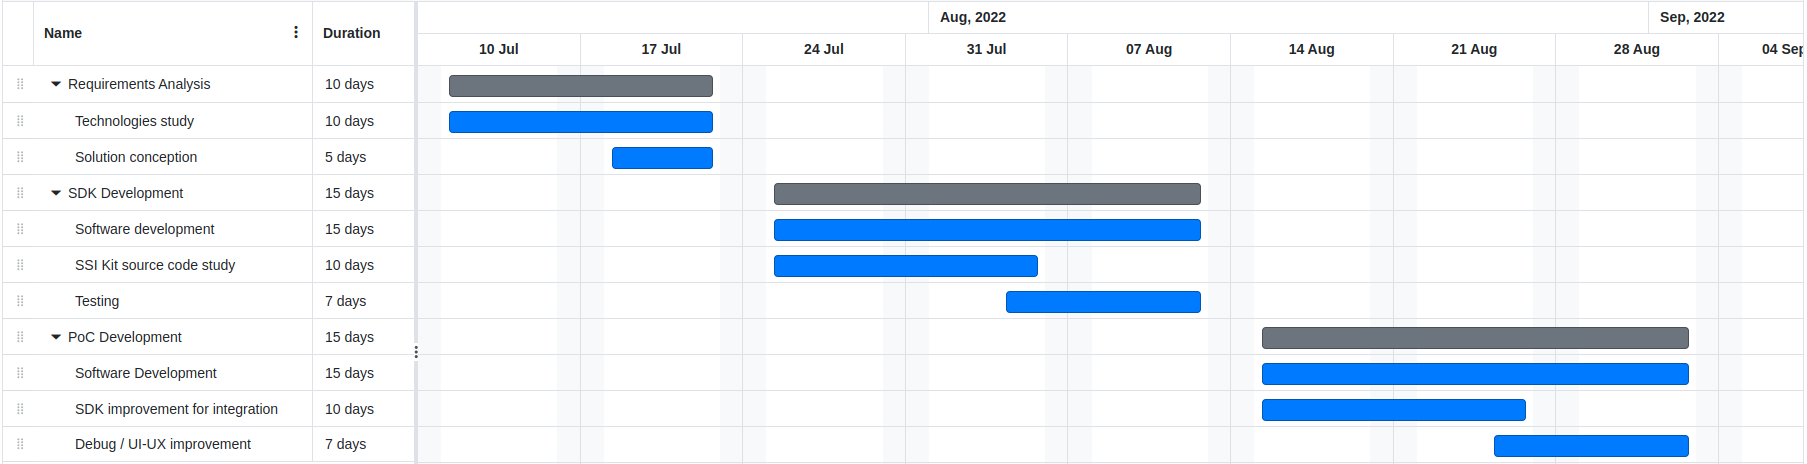
\includegraphics[keepaspectratio = true, width=15cm]{chapter1/internshipGantt.png}
    \captionof{figure}{Internship schedule}
\end{center}
